%!TEX TS-program = pdflatex
%!TEX encoding = MacOSRoman

% Modello di presentazione di tesi al computer.
% Collaudato sia con LaTeX che con pdfLaTeX.
% Richide alcuni file di stile
% (marslide.sty marsdefs.sty mars-cds.sty hugefonts.sty)
% e alcune figure, che sono forniti insieme
% con questo file.
% Scritto da Gianluca Gorni
% Versione: 9 novembre 2006

\documentclass[12pt,italian,oneside]{report}

\usepackage{ifpdf}
\usepackage[italian]{babel}
\usepackage{uniudpres}
\usepackage[latin1]{inputenc}
\usepackage{pdfpages}
\usepackage{paralist}
\usepackage{bm}
\usepackage{mathrsfs}

\graphicspath{{./figure/}}

\newcounter{cap}
\setcounter{cap}{2}
\newtheorem{definiz}{Definizione}[cap]
\newtheorem{defin}[definiz]{Definizione}
\newtheorem{teor}[definiz]{Teorema}
\newtheorem{teo}{Teorema}

%% Da usare con pdfLaTeX
%% per l'eventuale conversione automatica
%% delle figure da eps in pdf:
% \usepackage{epstopdf} 
\hyperbaseurl{http://www.dimi.uniud.it/gorni/TeX/itTeXdoc/}

%% Impostazioni del documento pdf (non essenziali,
%% ma non guastano):
\hypersetup{
  % bookmarksopenlevel=2, % default
  % pdfpagelayout=SinglePage, % default
  % pdfpagemode=FullScreen, % default
  pdftitle={Progettazione e sviluppo di un'applicazione mobile cross platform per il monitoraggio di dati nautici},
  pdfauthor={Federico Zanardo},
  pdfsubject={},
  pdfkeywords={}}
  % queste informazioni su titolo-autore-soggetto-parole chiave non vengono stampate, ma sono conservate nel documento pdf (premere command-D per vederle sotto AdobeReader/AcrobatReader). Tornano buone a scopi archivistici.

% Comandi per i colori:
\newcommand{\nero}[1]{\textcolor{black}{#1}}
\newcommand{\rosso}[1]{\textcolor{red}{#1}}
\newcommand{\verdescuro}[1]{\textcolor{darkgreen}{#1}}
\newcommand{\blu}[1]{\textcolor{blue}{#1}}
\definecolor{ocra}{rgb}{.45,.24,.1}
\newcommand{\ocra}[1]{\textcolor{ocra}{#1}}
\newcommand{\sfondogiallo}[1]{\colorbox{yellow}{#1}}
\newcommand{\displaysfondogiallo}[1]{\begin{center}%
  \sfondogiallo{$\displaystyle{#1}$}\end{center}}

% Informazioni per l'intestazione
\laureando{Federico Zanardo}
\relatore[Prof.]{Ivan Scagnetto}
%\corsodilaurea{Matematica} % vecchio ordinamento
 \corsodilaureatriennale{Informatica}
% \corsodilaureaspecialistica{Fisica Computazionale}
\titolo{\huge Progettazione e sviluppo di\\ \huge un'applicazione mobile cross\\ \huge platform per il monitoraggio\\ \huge di dati nautici}
\data{16 Luglio 2020}
%\dedica{A chi mi pare}
\correlatore[Prof.]{Francesco Trevisan}
%\ignorapause
%%%%%%%%%%%%%%%%%%%%%%%%%%%%%%%%%%%%%%%%%%%%%%%%%%%%%%%
\begin{document}

\maketitle

\raggedright

%\tableofcontents
% Provare come viene l'indice a doppia colonna:
% \indicedoppiacolonna

%\chapter{Progettazione e sviluppo\label{intestazioneCapitolo}}

%%%%%%%%%%%%%%%%%%%%%%%%%%%%%%%%%%%%%%%%%

\section{Progettazione e Sviluppo}

\begin{firstheadlineitemize}
	\item Requisiti per l'architettura
	\begin{secondheadlineitemize}
		\item Flessibile
		\item Strutturata
		\item Facile da utilizzare per implementare funzionalita' future
	\end{secondheadlineitemize}

	\item Architettura stratificata
	\begin{figure}[htp]
		\centering
		\hfill
		\begin{minipage}[b]{.3\columnwidth}
			%\centering
			\footnotesize
			\begin{secondheadlineitemize}
				\item \rosso{BLoC}
				\item Repository
			\end{secondheadlineitemize}
		\end{minipage}
		%\hfill
		\begin{minipage}[c]{.5\columnwidth}
			\begin{center}
				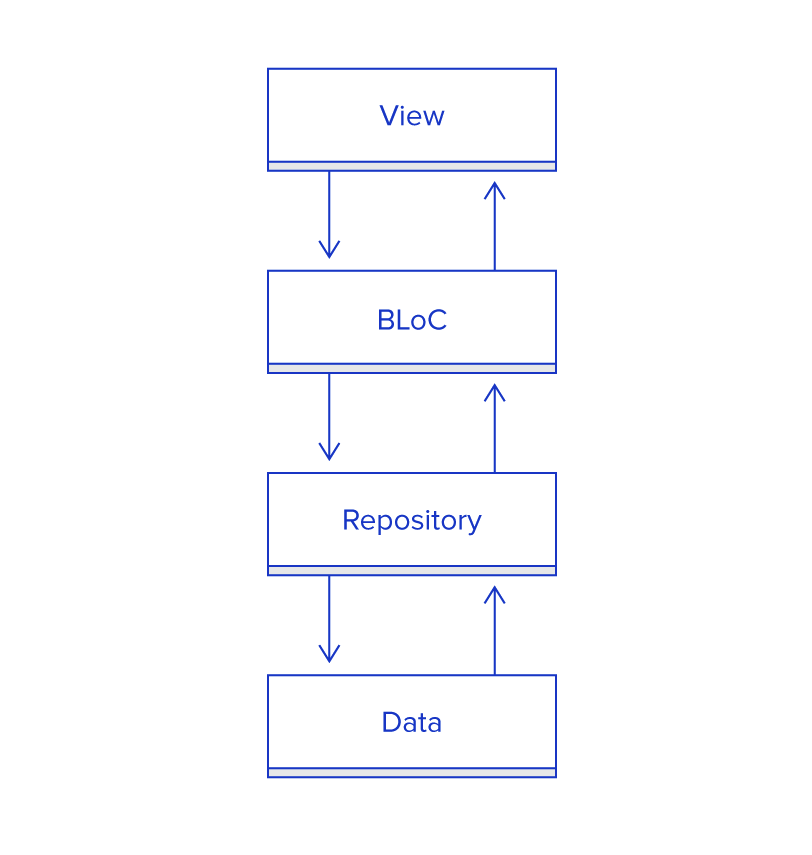
\includegraphics[scale=0.25]{architettura_implementata}
			\end{center}
		\end{minipage}\hspace*{\fill}
	\end{figure}
\end{firstheadlineitemize}

\newpage

\begin{firstheadlineitemize}

\item Interfaccia grafica

\begin{figure}[htp]
	\centering
	\hfill
	\begin{minipage}[c]{.3\columnwidth}
		\centering
	  	\begin{secondheadlineitemize}
			\item \rosso{Intuitiva}
			\item Organizzata
			\item Semplice
			\item \rosso{Reattiva}
		\end{secondheadlineitemize}
	\end{minipage}
	%\hfill
	\begin{minipage}[c]{.5\columnwidth}
	%  \begin{figure}[htp]
		%\centering
		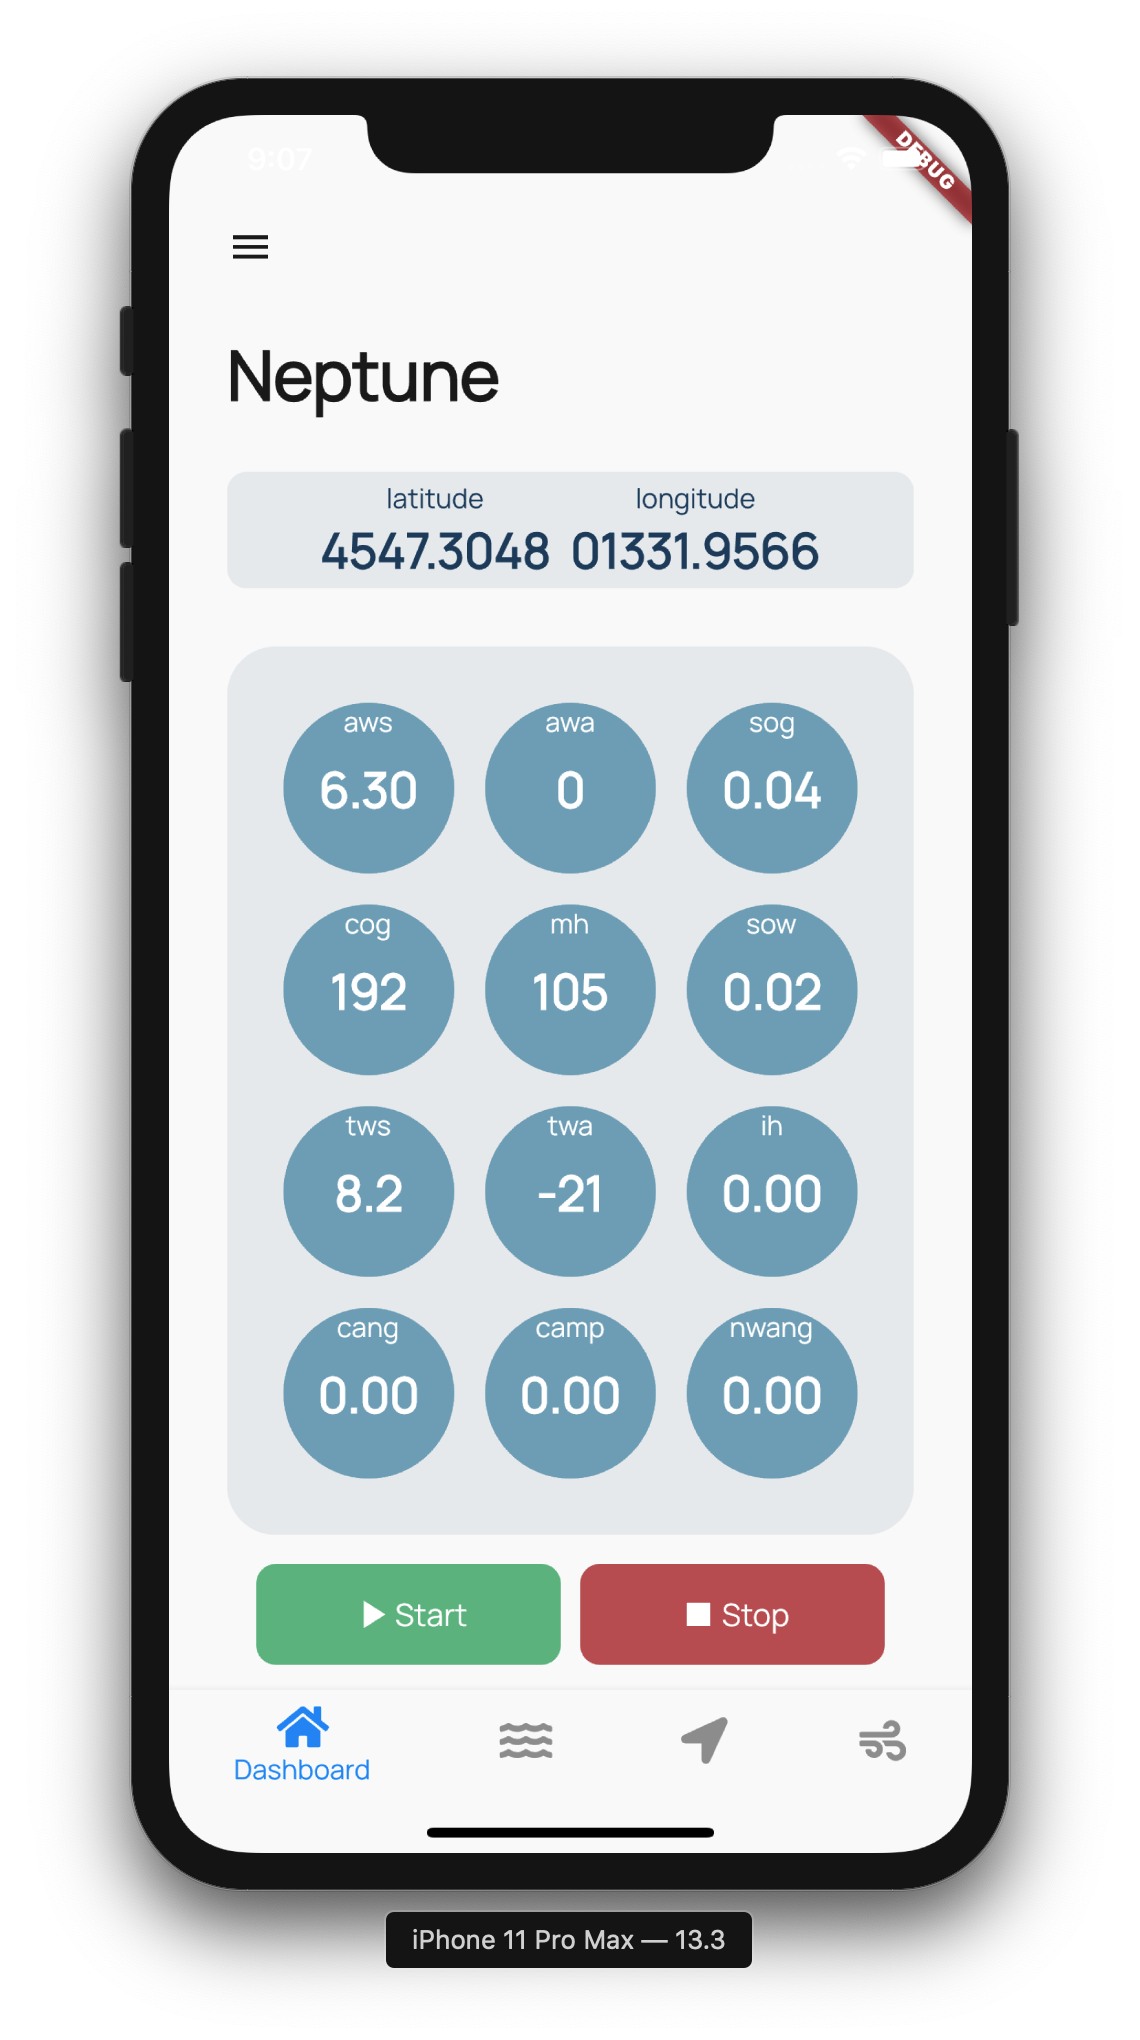
\includegraphics[scale=0.31]{dashboard}
		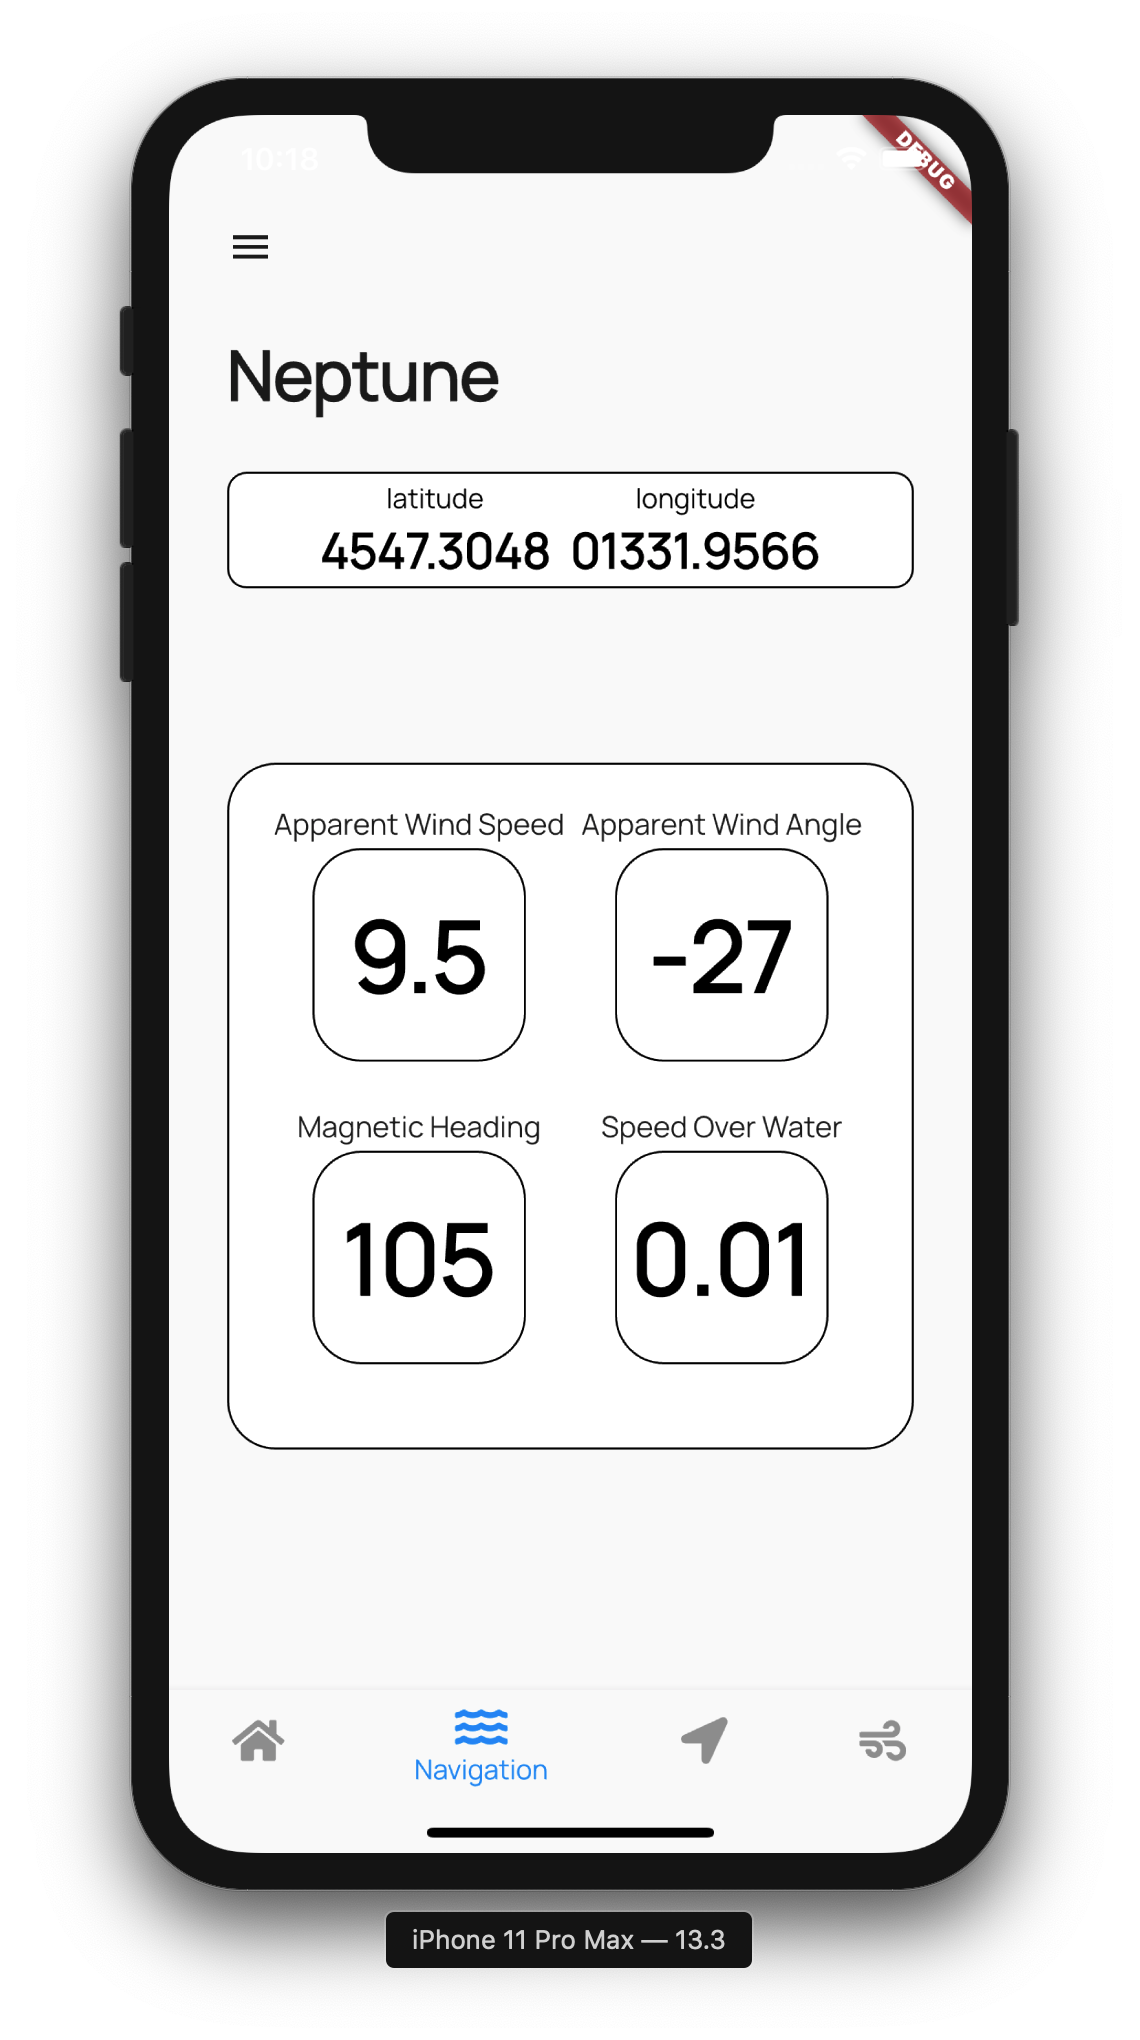
\includegraphics[scale=0.31]{navigation_high_contrast}
	%\end{figure}
	\end{minipage}\hspace*{\fill}
\end{figure}

\end{firstheadlineitemize}

%\pageTransitionBoxI

\end{document}